\chapter{Evaluation}

\section{Performance Evaluation}
\label{sec:performance-comparison}

Our evaluation aims to answer the following research questions:

\begin{itemize}

\item {\textbf{RQ1:}} Does adding scheduling to Vericert lead to a significant improvement in the quality of the generated hardware (in terms of area and delay)?

\item {\textbf{RQ2:}} Is hyperblock scheduling better than na\"ive list scheduling?

\item {\textbf{RQ3:}} Does adding scheduling make Vericert competitive with unverified HLS tools?

\item {\textbf{RQ4:}} Did our design decisions (e.g. \cref{sec:thirdattempt}) lead to an acceptable compilation time?

\end{itemize}

\definecolor{colorVericertBase}{HTML}{66c2a5}
\definecolor{colorVericertList}{HTML}{fc8d62}
\definecolor{colorVericertHyper}{HTML}{8da0cb}
\definecolor{colorBambuNoOpt}{HTML}{e78ac3}
\definecolor{colorBambuDefault}{HTML}{bbbbbb}

\colorlet{colorVericertBaseLIGHT}{colorVericertBase!50!white}
\colorlet{colorVericertListLIGHT}{colorVericertList!50!white}
\colorlet{colorVericertHyperLIGHT}{colorVericertHyper!50!white}
\colorlet{colorBambuNoOptLIGHT}{colorBambuNoOpt!50!white}
\colorlet{colorBambuDefaultLIGHT}{colorBambuDefault!50!white}

\newcommand\BambuDefault{%
\setul{-1pt}{3pt}\setulcolor{colorBambuDefaultLIGHT}%
{\ul{\textsf{Bambu-default}}}}

\newcommand\BambuNoOpt{%
\setul{-1pt}{3pt}\setulcolor{colorBambuNoOptLIGHT}%
{\ul{\textsf{Bambu-no-opt}}}}

\newcommand\VericertBase{%
\setul{-1pt}{3pt}\setulcolor{colorVericertBaseLIGHT}%
{\ul{\textsf{Vericert-original}}}}

\newcommand\VericertList{%
\setul{-1pt}{3pt}\setulcolor{colorVericertListLIGHT}%
{\ul{\textsf{Vericert-list-scheduling}}}}

\newcommand\VericertHyper{%
\setul{-1pt}{3pt}\setulcolor{colorVericertHyperLIGHT}%
{\ul{\textsf{Vericert-hyperblock-scheduling}}}}

\begin{figure*}
  \centering
  \resizebox{\linewidth}{!}{% GNUPLOT: LaTeX picture with Postscript
\begingroup
  \makeatletter
  \providecommand\color[2][]{%
    \GenericError{(gnuplot) \space\space\space\@spaces}{%
      Package color not loaded in conjunction with
      terminal option `colourtext'%
    }{See the gnuplot documentation for explanation.%
    }{Either use 'blacktext' in gnuplot or load the package
      color.sty in LaTeX.}%
    \renewcommand\color[2][]{}%
  }%
  \providecommand\includegraphics[2][]{%
    \GenericError{(gnuplot) \space\space\space\@spaces}{%
      Package graphicx or graphics not loaded%
    }{See the gnuplot documentation for explanation.%
    }{The gnuplot epslatex terminal needs graphicx.sty or graphics.sty.}%
    \renewcommand\includegraphics[2][]{}%
  }%
  \providecommand\rotatebox[2]{#2}%
  \@ifundefined{ifGPcolor}{%
    \newif\ifGPcolor
    \GPcolortrue
  }{}%
  \@ifundefined{ifGPblacktext}{%
    \newif\ifGPblacktext
    \GPblacktexttrue
  }{}%
  % define a \g@addto@macro without @ in the name:
  \let\gplgaddtomacro\g@addto@macro
  % define empty templates for all commands taking text:
  \gdef\gplbacktext{}%
  \gdef\gplfronttext{}%
  \makeatother
  \ifGPblacktext
    % no textcolor at all
    \def\colorrgb#1{}%
    \def\colorgray#1{}%
  \else
    % gray or color?
    \ifGPcolor
      \def\colorrgb#1{\color[rgb]{#1}}%
      \def\colorgray#1{\color[gray]{#1}}%
      \expandafter\def\csname LTw\endcsname{\color{white}}%
      \expandafter\def\csname LTb\endcsname{\color{black}}%
      \expandafter\def\csname LTa\endcsname{\color{black}}%
      \expandafter\def\csname LT0\endcsname{\color[rgb]{1,0,0}}%
      \expandafter\def\csname LT1\endcsname{\color[rgb]{0,1,0}}%
      \expandafter\def\csname LT2\endcsname{\color[rgb]{0,0,1}}%
      \expandafter\def\csname LT3\endcsname{\color[rgb]{1,0,1}}%
      \expandafter\def\csname LT4\endcsname{\color[rgb]{0,1,1}}%
      \expandafter\def\csname LT5\endcsname{\color[rgb]{1,1,0}}%
      \expandafter\def\csname LT6\endcsname{\color[rgb]{0,0,0}}%
      \expandafter\def\csname LT7\endcsname{\color[rgb]{1,0.3,0}}%
      \expandafter\def\csname LT8\endcsname{\color[rgb]{0.5,0.5,0.5}}%
    \else
      % gray
      \def\colorrgb#1{\color{black}}%
      \def\colorgray#1{\color[gray]{#1}}%
      \expandafter\def\csname LTw\endcsname{\color{white}}%
      \expandafter\def\csname LTb\endcsname{\color{black}}%
      \expandafter\def\csname LTa\endcsname{\color{black}}%
      \expandafter\def\csname LT0\endcsname{\color{black}}%
      \expandafter\def\csname LT1\endcsname{\color{black}}%
      \expandafter\def\csname LT2\endcsname{\color{black}}%
      \expandafter\def\csname LT3\endcsname{\color{black}}%
      \expandafter\def\csname LT4\endcsname{\color{black}}%
      \expandafter\def\csname LT5\endcsname{\color{black}}%
      \expandafter\def\csname LT6\endcsname{\color{black}}%
      \expandafter\def\csname LT7\endcsname{\color{black}}%
      \expandafter\def\csname LT8\endcsname{\color{black}}%
    \fi
  \fi
    \setlength{\unitlength}{0.0500bp}%
    \ifx\gptboxheight\undefined%
      \newlength{\gptboxheight}%
      \newlength{\gptboxwidth}%
      \newsavebox{\gptboxtext}%
    \fi%
    \setlength{\fboxrule}{0.5pt}%
    \setlength{\fboxsep}{1pt}%
    \definecolor{tbcol}{rgb}{1,1,1}%
\begin{picture}(10800.00,7200.00)%
    \gplgaddtomacro\gplbacktext{%
      \csname LTb\endcsname%%
      \put(518,5449){\makebox(0,0)[r]{\strut{}1}}%
      \csname LTb\endcsname%%
      \put(518,5766){\makebox(0,0)[r]{\strut{}2}}%
      \csname LTb\endcsname%%
      \put(518,5951){\makebox(0,0)[r]{\strut{}3}}%
      \csname LTb\endcsname%%
      \put(518,6185){\makebox(0,0)[r]{\strut{}5}}%
      \csname LTb\endcsname%%
      \put(518,6501){\makebox(0,0)[r]{\strut{}10}}%
      \csname LTb\endcsname%%
      \put(518,6920){\makebox(0,0)[r]{\strut{}25}}%
    }%
    \gplgaddtomacro\gplfronttext{%
      \csname LTb\endcsname%%
      \put(161,6202){\rotatebox{-270}{\makebox(0,0){\strut{}Relative execution time}}}%
    }%
    \gplgaddtomacro\gplbacktext{%
      \csname LTb\endcsname%%
      \put(518,3477){\makebox(0,0)[r]{\strut{}1}}%
      \csname LTb\endcsname%%
      \put(518,3811){\makebox(0,0)[r]{\strut{}2}}%
      \csname LTb\endcsname%%
      \put(518,4007){\makebox(0,0)[r]{\strut{}3}}%
      \csname LTb\endcsname%%
      \put(518,4253){\makebox(0,0)[r]{\strut{}5}}%
      \csname LTb\endcsname%%
      \put(518,4587){\makebox(0,0)[r]{\strut{}10}}%
      \csname LTb\endcsname%%
      \put(518,5029){\makebox(0,0)[r]{\strut{}25}}%
    }%
    \gplgaddtomacro\gplfronttext{%
      \csname LTb\endcsname%%
      \put(161,4228){\rotatebox{-270}{\makebox(0,0){\strut{}Relative cycle count}}}%
    }%
    \gplgaddtomacro\gplbacktext{%
      \csname LTb\endcsname%%
      \put(616,1546){\makebox(0,0)[r]{\strut{}0.7}}%
      \csname LTb\endcsname%%
      \put(616,1855){\makebox(0,0)[r]{\strut{}1.0}}%
      \csname LTb\endcsname%%
      \put(616,2455){\makebox(0,0)[r]{\strut{}2.0}}%
      \csname LTb\endcsname%%
      \put(616,2806){\makebox(0,0)[r]{\strut{}3.0}}%
      \csname LTb\endcsname%%
      \put(616,3055){\makebox(0,0)[r]{\strut{}4.0}}%
      \csname LTb\endcsname%%
      \put(888,1448){\rotatebox{-90}{\makebox(0,0)[l]{\strut{}2mm}}}%
      \csname LTb\endcsname%%
      \put(1237,1448){\rotatebox{-90}{\makebox(0,0)[l]{\strut{}3mm}}}%
      \csname LTb\endcsname%%
      \put(1586,1448){\rotatebox{-90}{\makebox(0,0)[l]{\strut{}adi}}}%
      \csname LTb\endcsname%%
      \put(1935,1448){\rotatebox{-90}{\makebox(0,0)[l]{\strut{}atas}}}%
      \csname LTb\endcsname%%
      \put(2284,1448){\rotatebox{-90}{\makebox(0,0)[l]{\strut{}bicg}}}%
      \csname LTb\endcsname%%
      \put(2633,1448){\rotatebox{-90}{\makebox(0,0)[l]{\strut{}cholesky}}}%
      \csname LTb\endcsname%%
      \put(2982,1448){\rotatebox{-90}{\makebox(0,0)[l]{\strut{}covariance}}}%
      \csname LTb\endcsname%%
      \put(3331,1448){\rotatebox{-90}{\makebox(0,0)[l]{\strut{}doitgen}}}%
      \csname LTb\endcsname%%
      \put(3680,1448){\rotatebox{-90}{\makebox(0,0)[l]{\strut{}durbin}}}%
      \csname LTb\endcsname%%
      \put(4029,1448){\rotatebox{-90}{\makebox(0,0)[l]{\strut{}fdtd-2d}}}%
      \csname LTb\endcsname%%
      \put(4378,1448){\rotatebox{-90}{\makebox(0,0)[l]{\strut{}floyd-warshall}}}%
      \csname LTb\endcsname%%
      \put(4727,1448){\rotatebox{-90}{\makebox(0,0)[l]{\strut{}gemm}}}%
      \csname LTb\endcsname%%
      \put(5076,1448){\rotatebox{-90}{\makebox(0,0)[l]{\strut{}gemver}}}%
      \csname LTb\endcsname%%
      \put(5425,1448){\rotatebox{-90}{\makebox(0,0)[l]{\strut{}gesummv}}}%
      \csname LTb\endcsname%%
      \put(5774,1448){\rotatebox{-90}{\makebox(0,0)[l]{\strut{}heat-3d}}}%
      \csname LTb\endcsname%%
      \put(6123,1448){\rotatebox{-90}{\makebox(0,0)[l]{\strut{}jacobi-1d}}}%
      \csname LTb\endcsname%%
      \put(6472,1448){\rotatebox{-90}{\makebox(0,0)[l]{\strut{}jacobi-2d}}}%
      \csname LTb\endcsname%%
      \put(6821,1448){\rotatebox{-90}{\makebox(0,0)[l]{\strut{}lu}}}%
      \csname LTb\endcsname%%
      \put(7170,1448){\rotatebox{-90}{\makebox(0,0)[l]{\strut{}ludcmp}}}%
      \csname LTb\endcsname%%
      \put(7519,1448){\rotatebox{-90}{\makebox(0,0)[l]{\strut{}mvt}}}%
      \csname LTb\endcsname%%
      \put(7868,1448){\rotatebox{-90}{\makebox(0,0)[l]{\strut{}nussinov}}}%
      \csname LTb\endcsname%%
      \put(8217,1448){\rotatebox{-90}{\makebox(0,0)[l]{\strut{}seidel-2d}}}%
      \csname LTb\endcsname%%
      \put(8566,1448){\rotatebox{-90}{\makebox(0,0)[l]{\strut{}symm}}}%
      \csname LTb\endcsname%%
      \put(8915,1448){\rotatebox{-90}{\makebox(0,0)[l]{\strut{}syr2k}}}%
      \csname LTb\endcsname%%
      \put(9264,1448){\rotatebox{-90}{\makebox(0,0)[l]{\strut{}syrk}}}%
      \csname LTb\endcsname%%
      \put(9613,1448){\rotatebox{-90}{\makebox(0,0)[l]{\strut{}trisolv}}}%
      \csname LTb\endcsname%%
      \put(9962,1448){\rotatebox{-90}{\makebox(0,0)[l]{\strut{}trmm}}}%
      \csname LTb\endcsname%%
      \put(10311,1448){\rotatebox{-90}{\makebox(0,0)[l]{\strut{}median}}}%
    }%
    \gplgaddtomacro\gplfronttext{%
      \csname LTb\endcsname%%
      \put(161,2300){\rotatebox{-270}{\makebox(0,0){\strut{}Relative area}}}%
      \csname LTb\endcsname%%
      \put(9730,2896){\makebox(0,0)[r]{\strut{}\footnotesize Vericert-original}}%
      \csname LTb\endcsname%%
      \put(9730,2720){\makebox(0,0)[r]{\strut{}\footnotesize Vericert-list-scheduling}}%
      \csname LTb\endcsname%%
      \put(9730,2545){\makebox(0,0)[r]{\strut{}\footnotesize Vericert-hyperblock-scheduling}}%
      \csname LTb\endcsname%%
      \put(9730,2369){\makebox(0,0)[r]{\strut{}\footnotesize Bambu-no-opt}}%
    }%
    \gplbacktext
    \put(0,0){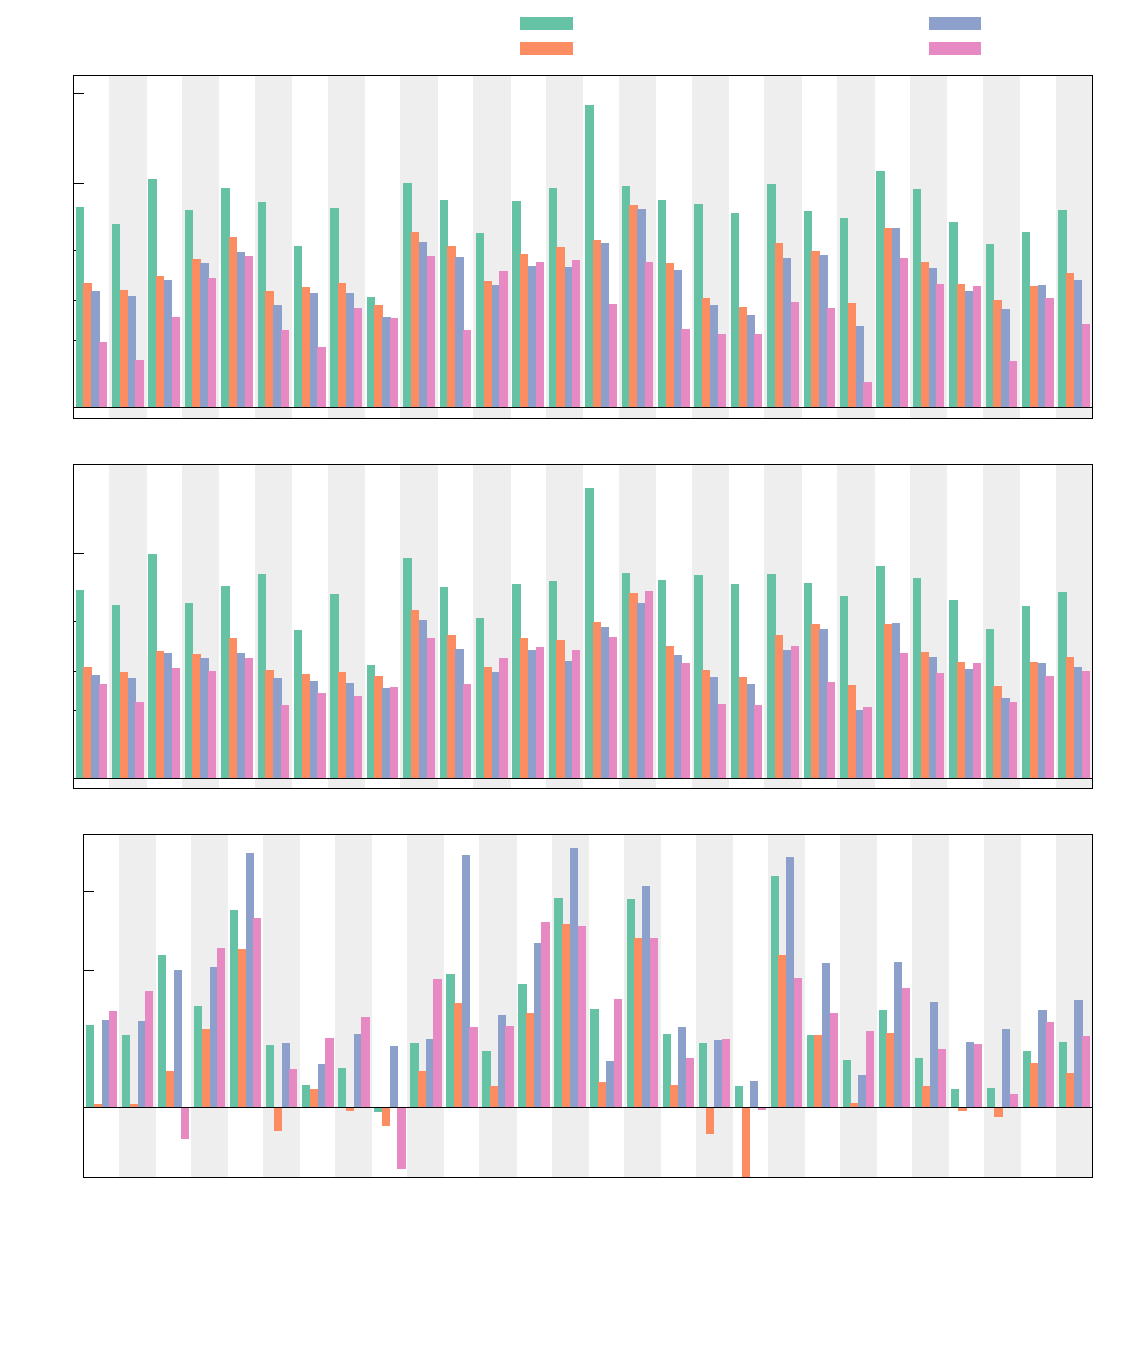
\includegraphics[width={540.00bp},height={360.00bp}]{bar-plot}}%
    \gplfronttext
  \end{picture}%
\endgroup
}
  \caption{Results of simulating and synthesising the PolyBench/C benchmark suite using a range of HLS tools. All figures are relative to \BambuDefault{}.}%
  \label{fig:list-against-hyper-scheduling}
\end{figure*}

\paragraph{Experimental setup}
Following \textcite{herklotz21_formal_verif_high_level_synth} and \textcite{six22_formal_verif_super_sched}, we evaluate our work using PolyBench/C~\cite{pouchet20_polyb_c}. For each benchmark, the resulting Verilog hardware design was simulated using Verilator to get the total cycle count. Each design was synthesised, placed, and routed onto a Xilinx series 7 FPGA (part number: \mono{xc7z020clg484-1}) using Vivado to get its total area and its maximum frequency.
We then calculated $\text{total execution time} = \frac{\text{total clock cycles}}{\text{maximum frequency}}$.  We ensured that every design met the timing constraints of a 100MHz clock.

\paragraph{Answering RQ1}
To assess whether adding scheduling to Vericert leads to better hardware designs, \cref{fig:list-against-hyper-scheduling} compares the hardware produced by original Vericert (\VericertBase{}) with that produced when hyperblock scheduling is enabled (\VericertHyper{}). We see that, on average, hyperblock scheduling leads to hardware that requires only 0.46$\times$ the cycle count (middle plot). This is unsurprising given that original Vericert only executed a single instruction per clock cycle. In terms of area (bottom plot), hyperblock scheduling has, on average, a slight increase in area.

\paragraph{Answering RQ2}
Hyperblock scheduling is considerably more complicated to implement and verify than list scheduling, as it requires if-conversion to combine basic blocks into hyperblocks, as well as predicate-aware scheduling. If we omit if-conversion entirely (hence avoiding predication too), we obtain list scheduling as a special case. Does hyperblock scheduling yield enough of a performance improvement over list scheduling to justify its additional complexity?

To answer this, \cref{fig:list-against-hyper-scheduling} measures the hardware produced by Vericert with list scheduling (\VericertList{}). On average, list scheduling leads to hardware that requires 0.51$\times$ the cycle count compared to \VericertBase{}, which is 1.1$\times$ the cycle count compared to \VericertHyper{}. We expect hyperblock scheduling to extend its small lead over list scheduling once the heuristics that guide if-conversion are improved.  In particular, our predictions of the latency of predicated instructions are currently quite conservative to ensure that timing constraints are met; improving these estimates is an active research area~\cite{TanFeb15,RizziJul23,WangOct23,UstunNov20,ZhengFeb14}.

In terms of area, we see that \VericertList{} leads to the smallest hardware designs. This can be attributed to the downstream logic synthesis tool being able to save area by optimising chained operations, such as multiply--accumulate, while not having to handle the predicates that are introduced with \VericertHyper{}.

\paragraph{Answering RQ3}
To assess how \VericertHyper{} fares against unverified HLS tools, we compare it against the state-of-the-art open-source HLS tool Bambu~\cite[]{ferrandi2021bambu}. We use Bambu in two modes: one where all default optimisations are enabled (\BambuDefault{}), and one where as many optimisations as possible are disabled (\BambuNoOpt{}). Note that several `optimisations' are built into Bambu and cannot be disabled, such as list scheduling and loop flattening.

All the bars in \cref{fig:list-against-hyper-scheduling} are relative to \BambuDefault. The pink bars show \BambuNoOpt. We see that although \VericertHyper{} is well behind \BambuDefault{} (its designs require 3$\times$ the cycle count), it performs comparably to \BambuNoOpt{} (1.04$\times$ the cycle count), which is encouraging because \VericertHyper{} and \BambuNoOpt{} have similar feature sets.

\paragraph{Answering RQ4}
To assess whether \VericertHyper{} has acceptable compilation times, we also compare it against Bambu.  Compilation times did not deviate for Bambu, all of them being around 3s mainly due to long startup costs. \VericertHyper{} compiled each benchmark in 0.9s, also without much variation, showing that verification was not overly costly.  As for whether our design decisions led to these compilation times: we remark that if we disable the `final-state predicates' innovation that we introduced in \cref{sec:thirdattempt}, none of the benchmarks compile within a few minutes and eventually the machine runs out of memory.

% \Cref{fig:list-against-hyper-scheduling} shows the final results relative to the base version of Vericert.  First, the relative cycle counts between each tool shows that list scheduling has 0.59$\times$ the number of cycles compared to base Vericert and hyperblock scheduling has 0.56$\times$ the number of cycles compared to base Vericert, showing that scheduling instructions provides a large improvement compared to the total number of cycles of base Vericert.  Bambu with optimisations turned-off has around 0.42$\times$ the number of cycles, and with optimisations has 0.14$\times$ the number of cycles, taking drastically fewer cycles.  One outlier here is the jacobi-1d benchmark, where only optimised Bambu finds a way to reduce the number of cycles.  This is because it is a very small benchmark with a single loop, which cannot be optimised by the scheduling algorithms and requires more advanced loop optimisations such as loop pipelining.

% However, looking at the relative execution time is a bit surprising, because on average, the hyperblock scheduling algorithm only performs as well as base Vericert, whereas the list scheduling algorithm performs much better.  This is because the operation chaining heuristics used did not work consistently for the hyperblock scheduling pass, therefore reducing the maximum operating frequency dramatically in some cases.  This is something that needs to be addressed in the heuristics used to perform the if-conversion, but also in the latency constraints in the scheduler.  Interestingly, however, the output of the list scheduling algorithm is around 14\% faster than unoptimised Bambu.  Again, optimised Bambu optimises the benchmarks much further, but also has a slightly higher maximum frequency, bringing the gap down a bit compared to the total cycle counts.

% Finally, looking at area, list scheduling actually also reduces the area
% compared to base Vericert, which is mainly due to the synthesis tool being
% able to optimise chained operations, such as multiply-accumulate operations,
% further.  However, because of the addition of predicates in hyperblock
% scheduling, the area is similar to base Vericert.  This area is similar to
% unoptimised Bambu, however, optimised Bambu achieves 0.6$\times$ the area.

\section{Limitations and Future Work}

There are various limitations in \vericert{} compared to other HLS tools due to the fact that our main focus was on formally verifying the translation from 3AC to Verilog. In this section, we outline the current limitations of our tool and suggest how they can be overcome in future work, first describing limitations to the generated hardware, and then describing the limitations on the software input that \vericert{} accepts.

%\NR{You have very different types of limitations. I wonder if grouped them into software and hardware limitations respectively might simplify this section. Just a suggestion.}

\subsection{Limitations to the Generated Hardware}

%This section describes the current limitations and possible improvements that could be made to the generated hardware.

\paragraph{Lack of instruction-level parallelism}

%\JW{I'm hesitant about this paragraph. Yes, we have to write something about how future-proof Vericert is, as this is required by the reviewers and promised in our list of changes. But I worry that if we place too much emphasis on how straightforward it will be to add scheduling, then we'll make it harder for ourselves to publish a paper about adding scheduling (``But you said in your OOPSLA 2021 paper that this was all straightforward'' etc.) In what follows, I've tried to strike a balance -- see what you think.}\YH{Yeah I think I like the paragraph and the balance in it, I think it still explains that existing passes should not have to change.  I think reviewer 2 wanted a detailed explanation of this, but I do agree that it should not be needed in this paper.}
The main limitation of \vericert{} is that it does not perform instruction scheduling, which means that instructions cannot be gathered into the same state and executed in parallel.
%This limitation is present by design so that the focus could be made on the initial proof of correctness of the translation of instructions with a sequential schedule.
However, each language in \vericert{} was designed with scheduling in mind, so that these should not have to change fundamentally when that is implemented in the future.
For instance, our HTL language already allows arbitrary Verilog to appear in each state of the FSMD; currently, each state just contains a single Verilog assignment, but when scheduling is added, it will contain a list of assignments that can all be executed in parallel. We expect to follow the lead of \textcite{tristan08_formal_verif_trans_valid} and \textcite{six+20}, who have previously added scheduling support to CompCert in a VLIW context, by invoking an external (unverified) scheduling tool and then using translation validation to verify that each generated schedule is correct (as opposed to verifying the scheduling tool itself).
%The translation from 3ACPar to HTL would not change conceptually, except for the fact that multiple instructions can now be translated into the same state.
%This means that the proof of translation from 3AC to HTL can also be adapted with minimal changes to the top-level of the proofs.
%The bulk of the proofs proving the translation of single instructions would stay intact.

%However, the design of the intermediate languages in \vericert{} take this optimisation into account and are designed to support scheduling in the future.

%\NRIt is best to explain why we didn't focus on scheduling with a positive/future work spin. For example, ``It was more intuitive to handle one instruction per cycle at the initial stage of our project as we want to focus our efforts on correctness, which has been the main weakness of HLS, rather than performance. However, we were very much aware during the design stage that in order for our compiler to be able to perform better, supporting of scheduling was inevitable. Hence, we intentionally left room for support of scheduling. In essence, instead of supporting one instruction per cycle, we must be able to support a list of instructions per cycle. To do so, we envision extensions to our work in several ways.'' We might not even need to specify the details of how. You can keep the tricks in your sleeves for the next publication. \YH{Well one of the only things the reviewers wanted us to add was a realistic implementation of scheduling, so I think we need to at least keep that.}.

%To simplify the proof of the scheduling algorithm, and to minimise the changes necessary for the current translation from 3AC to HTL, a new language must be introduced, called 3ACPar, which would be equivalent to 3AC but instead of consisting of a map from program counter to instruction, it would consist of a map from program counter to list of instructions, which can all be executed in parallel.  A new proof for the scheduling algorithm would have to be written for the translation from 3AC to 3ACPar, for which a verified translation validation approach might be appropriate, however, the translation form 3ACPar to HTL would not change conceptually, except for the fact that multiple instructions can now be translated into the same state.  This small difference means that most of the proof can be reused without any changes, as the translation of instructions was the main body of the proof and did not change.

\paragraph{Lack of pipelined division}
Pipelined operators can execute different stages of an operation in parallel, and thus perform several long-running operations simultaneously while sharing the same hardware.
The introduction of pipelined operators to \vericert{}, especially for division, would alleviate the slow clock speed observed in the \polybench{} benchmarks when divisions were included (Fig.~\ref{fig:polybench-div}). In HTL, pipelined operations could be represented in a similar fashion to load and store instructions, by using wires to communicate with an abstract computation block modelled in HTL and later replaced by a hardware implementation.
%\NR{Are you describing using IP blocks? If so, you can generalise it to any IP block rather than just division.}\YH{I think I prefer just focusing on pipelined division for now, as that's specifically the issue, so that people know we have a plan to resolve specifically that.}
%JW I've chopped the following sentence because it felt like it was going into too much detail.
%However, 3ACPar would have to be modified to also describe such instructions so that these can be placed optimally using the external scheduling algorithm.

\subsection{Limitations on the Software Input}

%This section describes the limitations and possible improvements to the software input accepted by \vericert{}.

\paragraph{Limitations with I/O}

\vericert{} is currently limited in terms of I/O because the main function cannot accept any arguments if the Clight program is to be well-formed.\footnote{Technically, \vericert{} (and indeed, \compcert{}) can compile main functions that have arbitrary arguments and will handle those inputs appropriately, but the correctness theorem offers no guarantees about such programs.} Moreover, external function calls that produce traces have not been implemented yet, but these could enable the C program to read and write values on a bus that is shared with various other components in the hardware design.

\paragraph{Lack of support for global variables}
In \compcert{}, each global variable is stored in its own memory.  A generalisation of our translation of the stack into a RAM block could therefore translate global variables in the same manner.  This would require a slight generalisation of pointers so that they store provenance information to ensure that each pointer accesses the right RAM. It would also be necessary to generalise the RAM interface so that it decodes the provenance information and indexes the correct array.
%\NR{Curiously, is memory analysis in your to-do list?}\YH{Well kind of, would be nice, but probably not sophisticated analysis.}

\paragraph{Other language restrictions}
C and Verilog handle signedness quite differently. By default, all operators and registers in Verilog (and HTL) are unsigned, so to force an operation to handle the bits as signed, both operators have to be forced to be signed. Moreover, Verilog implicitly resizes expressions to the largest needed size by default, which can affect the result of the computation.  This feature is not supported by the Verilog semantics we adopted, so to match the semantics to the behaviour of the simulator and synthesis tool, braces are placed around all expressions to inhibit implicit resizing.  Instead, explicit resizing is used in the semantics, and operations can only be performed on two registers that have the same size.

Furthermore, equality checks between \emph{unsigned} variables are actually not supported, because this requires supporting the comparison of pointers, which should only be performed between pointers with the same provenance.  In \vericert{} there is currently no way to determine the provenance of a pointer, and it therefore cannot model the semantics of unsigned comparison in \compcert{}. This is not a severe restriction in practice however, because in the absence of dynamic allocation, equality comparison of pointers is rarely needed, and equality comparison of integers can still be performed by casting them both to signed integers.

Finally, the \texttt{mulhs} and \texttt{mulhu} instructions, which fetch the
upper bits of a 32-bit multiplication, are not translated by \vericert{},
because 64-bit numbers are not supported. These instructions are only generated
to optimise divisions by a constant that is not a power of two, so turning off
constant propagation will allow these programs to pass without error.

\subsection{Coq Mechanisation}

\begin{table}
  \centering
  \caption{Statistics about the numbers of lines of code in the proof and implementation of \vericert{}.}\label{tab:proof_statistics}
  \begin{tabular}{lrrrrr}
    \toprule
    & \textbf{Coq code} & \multicolumn{1}{p{1cm}}{\raggedleft\textbf{OCaml code}} & \textbf{Spec} & \multicolumn{1}{p{2cm}}{\raggedleft\textbf{Theorems \& Proofs}} & \textbf{Total}\\
    \midrule
    {Data structures and libraries}     & 280  & --- & ---  & 500  & 780   \\
    {Integers and values}               & 98   & --- & 15   & 968  & 1081  \\
    {HTL semantics}                     & 50   & --- & 181  & 65   & 296   \\
    {HTL generation}                    & 590  & --- & 66   & 3069 & 3725  \\
    {RAM generation}                    & 253  & --- & ---  & 2793 & 3046  \\
    {Verilog semantics}                 & 78   & --- & 431  & 235  & 744   \\
    {Verilog generation}                & 104  & --- & ---  & 486  & 590   \\
    {Top-level driver, pretty printers} & 318  & 775 & ---  & 189  & 1282  \\
    \midrule
    \textbf{Total}                      & 1721 & 775 & 693  & 8355 & 11544 \\
    \bottomrule
  \end{tabular}
\end{table}

The lines of code for the implementation and proof of \vericert{} can be found
in Table~\ref{tab:proof_statistics}.  Overall, it took about 1.5 person-years to
build \vericert{} -- about three person-months on implementation and 15
person-months on proofs.  The largest proof is the correctness proof for the HTL
generation, which required equivalence proofs between all integer operations
supported by \compcert{} and those supported in hardware.  From the 3069 lines
of proof code in the HTL generation, 1189 are for the correctness proof of just
the load and store instructions.  These were tedious to prove correct because of
the substantial difference between the memory models used, and the need to prove
properties such as stores outside of the allocated memory being undefined, so
that a finite array could be used. In addition to that, since pointers in HTL
and Verilog are represented as integers, instead of as a separate `pointer' type
like in the \compcert{} semantics, it was painful to reason about them.  Many
new theorems had to be proven about them in \vericert{} to prove the conversion
from pointer to integer.  Moreover, the second-largest proof of the correct RAM
generation includes many proofs about the extensional equality of array
operations, such as merging arrays with different assignments.  As the negative
edge implies that two merges take place every clock cycle, the proofs about the
equality of the contents in memory and in the merged arrays become more tedious
too.

Looking at the trusted computing base of \vericert{}, the Verilog semantics is
431 lines of code.  This and the Clight semantics from \compcert{} are the only
parts of the compiler that need to be trusted.  The Verilog semantics
specification is therefore much smaller compared to the 1721 lines of the
implementation that are written in Coq, which are the verified parts of the HLS
tool, even when the Clight semantics are added.  In addition to that,
understanding the semantics specification is simpler than trying to understand
the translation algorithm. We conclude that the trusted base has been
successfully reduced.

%%% Local Variables:
%%% mode: latex
%%% TeX-master: "../thesis"
%%% TeX-engine: luatex
%%% End:
